\documentclass[10pt]{article} % Документ принадлежит классу article, а также будет печататься в 12 пунктов.
\usepackage{array} % Для титульника
\usepackage{ucs}
\usepackage[utf8x]{inputenc} % Включаем поддержку UTF8
\usepackage[russian]{babel}  % Включаем пакет для поддержки русского языка
\usepackage[left=2cm,right=2cm, top=2cm,bottom=2cm,bindingoffset=0cm]{geometry} % Отступы по краям страницы
\usepackage{amssymb,amsfonts,amsmath,mathtext,cite,enumerate,float} % Математические штуки
\usepackage{cmap} % чтобы работал поиск по PDF
\usepackage{graphicx} % для вставки картинок
\usepackage{epstopdf} 	

\usepackage{wrapfig} % Обтектание картинок текстом
\usepackage{caption}
\usepackage{subcaption}
 
%  для гиперссылок
\usepackage{xcolor}
\usepackage{hyperref}
\definecolor{linkcolor}{HTML}{191970} % цвет ссылок
\definecolor{urlcolor}{HTML}{191970} % цвет гиперссылок
\hypersetup{pdfstartview=FitH,  linkcolor=linkcolor,urlcolor=urlcolor, colorlinks=true}

\usepackage{pscyr} % Нормальные шрифты
\usepackage{setspace} % Для отступов между строк
%Это для формирования листингов
%%%%%%%%%%%%%%%%%%%%%%%%Листинги на MATLAB
\usepackage{listings}
\usepackage{color} %red, green, blue, yellow, cyan, magenta, black, white
\definecolor{mygreen}{RGB}{28,172,0} % color values Red, Green, Blue
\definecolor{mylilas}{RGB}{170,55,241}

\lstset{language=Matlab,
	breaklines=true,%
	morekeywords={matlab2tikz},
	keywordstyle=\color{blue},%
	morekeywords=[2]{1}, keywordstyle=[2]{\color{black}},
	identifierstyle=\color{black},%
	stringstyle=\color{mylilas},
	commentstyle=\color{mygreen},%
	showstringspaces=false,%without this there will be a symbol in the places where there is a space
	numbers=left,%
	numberstyle={\tiny \color{black}},% size of the numbers
	numbersep=9pt, % this defines how far the numbers are from the text
	emph=[1]{for,end,break},emphstyle=[1]\color{blue}, %some words to emphasise
	inputencoding=cp1251
	%emph=[2]{word1,word2}, emphstyle=[2]{style},    
}

%%%%%%%%%%%%%%%%%%%%%%%%%%%%%%%%%


\begin{document} % Начало документа

\title{{\large Распознавание образов. Лабораторная работа №4.} \\
	\textbf{\textquotedblleft Распознавание образов, описываемых бинарными признаками\textquotedblright}.\\
	%{\large Вариант 8 (а)}
	}
\date{}
\author{\textit{Выполнил}: студент 4 курса, группы 6.1 \\
	Суходолов Денис}
        
\maketitle

\begin{spacing}{1} % Для отступов между строк
\section*{Описание работы}
\textbf{Цель работы}: Синтезировать  алгоритмы  распознавания  образов,
описываемых  бинарными  признаками.  Исследовать  синтезированные
алгоритмы распознавания с точки зрения ожидаемых потерь и ошибок.
~\\
\textbf{Исходные данные:}
\begin{figure}[h]
	\centering
	\begin{subfigure}{.4\textwidth}
		\centering
		\includegraphics[width=.6\linewidth]{sphoto.eps}
		%\caption{A subfigure}
		%\label{fig:sub1}
	\end{subfigure}%
	\begin{subfigure}{.4\textwidth}
		\centering
		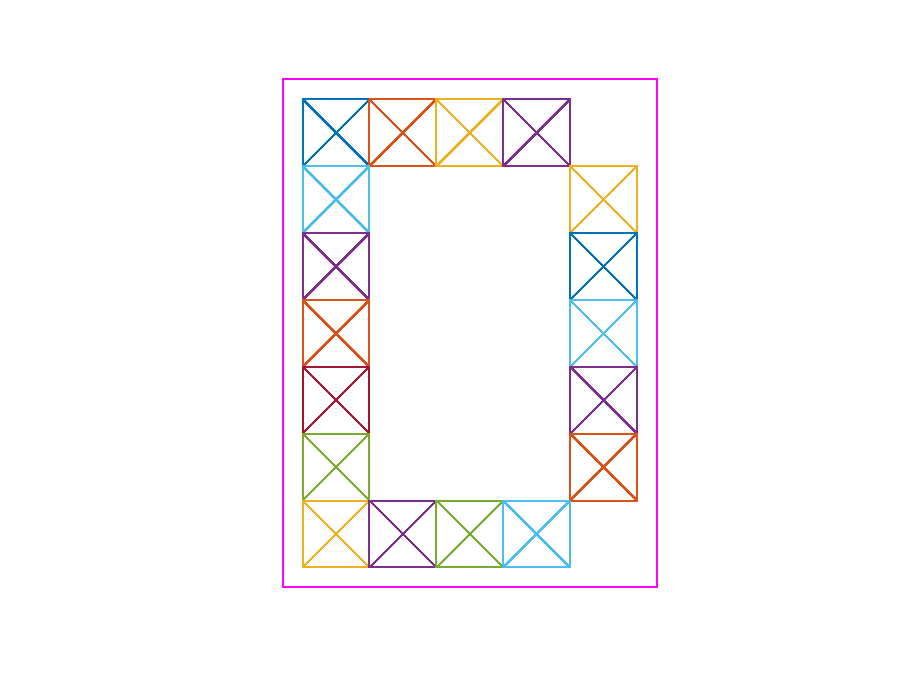
\includegraphics[width=.6\linewidth]{dphoto.eps}
		%\caption{A subfigure}
		%\label{fig:sub2}
	\end{subfigure}
	%\caption{A figure with two subfigures}
	%\label{fig:test}
\end{figure}
~\\
\textbf{Априорные вероятности классов:}
~\\
\begin{tabular}{| l | c | c |}
	\hline			
	Случай & $p(w_s)$ & $p(w_d)$ \\
	\hline	
	$p(w_s) > p(w_d)$ & 0.8 & 0.2 \\
	\hline	
	$p(w_s) = p(w_d)$ & 0.5 & 0.5 \\
	\hline  
	$p(w_s) < p(w_d)$ & 0.2 & 0.8 \\
	\hline  
\end{tabular}
~\\
~\\
\textbf{Код для задания разделяющей функции:}
\lstinputlisting[basicstyle=\ttfamily\footnotesize ]{razdel.m} 
\begin{figure}[h]
	\centering
	\begin{subfigure}{.5\textwidth}
		\centering
		\includegraphics[width=1.1\linewidth]{Sd1.eps}
		\caption{$p(w_s) > p(w_d)$}
		%\label{fig:sub1}
	\end{subfigure}%
	\begin{subfigure}{.5\textwidth}
		\centering
		\includegraphics[width=1.1\linewidth]{eqProb.eps}
		\caption{$p(w_s) = p(w_d)$}
		%\label{fig:sub2}
	\end{subfigure}
	\begin{subfigure}{.5\textwidth}
		\centering
		\includegraphics[width=1.1\linewidth]{sD2.eps}
		\caption{$p(w_s) < p(w_d)$}
		%\label{fig:sub2}
	\end{subfigure}
	\caption{Графики значений элементов теоретической и экспериментальной матриц вероятностей ошибок}
	%\label{fig:test}
\end{figure}
~\\
\textbf{Характер зависимости разделяющей функции от компонент вектора признаков} - линейный.














\end{spacing}
\end{document}